%%%%%
%%%%%  Naudokite LUALATEX, ne LATEX.
%%%%%
%%%%
\documentclass[]{VUMIFTemplateClass}
\usepackage{booktabs}
\usepackage{indentfirst}
\usepackage{amsmath, amsthm, amssymb, amsfonts}
\usepackage{mathtools}
\usepackage{physics}
\usepackage{graphicx}
\usepackage{verbatim}
\usepackage[hidelinks]{hyperref}
\usepackage{color,algorithm,algorithmic}
\usepackage[nottoc]{tocbibind}
\usepackage{tocloft}

\usepackage{titlesec}
\newcommand{\sectionbreak}{\clearpage}

\makeatletter
\renewcommand{\fnum@algorithm}{\thealgorithm}
\makeatother
\renewcommand\thealgorithm{\arabic{algorithm} algoritmas}

\usepackage{biblatex}
\bibliography{bibliografija}
%% norint pakeisti bibliografijos šaltinių numeravimą (skaitiniu arba raidiniu), pakeitimus atlikti VUMIFTemplateClass.cls 150 eilutėje

% Author's MACROS
\newcommand{\EE}{\mathbb{E}\,} % Mean
\newcommand{\ee}{{\mathrm e}}  % nice exponent
\newcommand{\RR}{\mathbb{R}}


\studijuprograma{Programų sistemų} %Studijų programą įrašyti kilmininko linksniu (pavyzdžiui – Programų sistemų, Finansų ir draudimų matematikos ir t. t.)
\darbopavadinimas{Praktinės informatikos pratybos}
\darbopavadinimasantras{(Practical Lesson in Practical Computer Science)}
\darbotipas{Kursinis darbas} % Bakalauro baigiamasis darbas arba magistro baigiamasis darbas
\autorius{1 kurso 1 grupės studentas Karolis Paškevičius}

%Autorių gali būti ir daugiau, tuo atveju, kiekvienas autorius rašomas iš naujos eilutės, ir pridedamas titulinis.tex arba dvigubasTitulinis.tex dokumentuose
%\antrasautorius{Vardas Pavardė} %Jei toks yra, kitu atveju ištrinti

\vadovas{Prof. Dr. Vytautas Čyras}

\begin{document}
\selectlanguage{lithuanian}

\onehalfspacing
\begin{titlepage}
\vskip 20pt
\begin{center}

\includegraphics[scale=0.55]{images/MIF.png}
\end{center}

\makeatletter

\vskip 20pt
\centerline{\bf \large \textbf{VILNIAUS UNIVERSITETAS}}
\vskip 10pt
\centerline{\large \textbf{MATEMATIKOS IR INFORMATIKOS FAKULTETAS}}
\vskip 10pt
\centerline{\large \textbf{\MakeUppercase{\@studijuprograma \space studijų programa}}}

\vskip 80pt
\centerline{\Large \@darbotipas}
\vskip 20pt
\begin{center}
    {\bf \LARGE \@darbopavadinimas}
\end{center}
\begin{center}
    {\bf \Large \@darbopavadinimasantras}
\end{center}
\vskip 80pt

\centering{
    \begin{tabular}{rcp{.7\textwidth}}
        {\Large Autorius} & {\Large :} & {\Large \@autorius}\\[10pt]
        \@ifundefined{@antrasautorius}{}
            {
                {\Large Antras autorius} & {\Large :} & {\Large \@antrasautorius}\\[10pt]
            }
    \end{tabular}}
\@ifundefined{@antrasautorius}{}
{
\vskip 10pt
\centering{\Large \@antrasautorius}
}
\vskip 20pt

\centering{
    \begin{tabular}{rcp{.7\textwidth}}
        {\Large Darbo vadovas} & {\Large :} & {\Large \@vadovas}\\[10pt]
        \@ifundefined{@moksliniskonsultantas}{}
            {
                {\Large Mokslinis konsultantas} & {\Large :} & {\Large \@moksliniskonsultantas}\\[10pt]
            }
        \@ifundefined{@recenzentas}{}
            {
                {\Large Recenzentas} & {\Large :} & {\Large \@recenzentas}\\[10pt]
            }
    \end{tabular}}


\vskip 110pt

\centerline{\large \textbf{Vilnius}}
\centerline{\large \textbf{\the\year{}}}

\makeatother

\newpage
\end{titlepage}
%\newgeometry{top=2cm,bottom=2cm,right=2cm,left=3cm}
\setcounter{page}{2}


%% Padėkų skyrius
\sectionnonumnocontent{Padėka}
Darbo autorius dėkoja Vilniaus universiteto Matematikos ir informatikos fakulteto Informacinių technologijų atviros prieigos centrui už suteiktus našiųjų skaičiavimų (angl. High Performance Computing, HPC) išteklius šio darbo tyrimui atlikti.
%%
%%
%%      Jei baigiamojo darbo tyrimui atlikti naudojote MIF suteikiamus IT išteklius (CPU-h, GPU-h, kitus IT resursus), padėką palikite, jei nenaudojote - galite ištrinti.
%%
%%

Čia taip pat galima pridėti padėkas įvairiems kitiems dalykams, pavyzdžiui: vadovui, universitetui, įmonei ir t. t.

%%Santrauka
\selectlanguage{lithuanian}
\sectionnonum{Santrauka}

Darbo santrauka.\\

\textbf{Raktiniai žodžiai:} čia surašomi su darbu susiję raktiniai žodžiai, \textit{\textbf{minimalus raktinių žodžių kiekis - 3}}, tačiau jų gali būti ir daugiau.


\sectionnonum{Summary}

Summary in english.\\

\textbf{Keywords:} work related keywords, with a \textit{\textbf{minimum of 3 keywords}}, but can be more.


\singlespacing

% iliustracijų sąrašas, jei jo nereikia - ištrinkite
\listoffigures 

%lentelių sąrašas, jei jo nereikia - ištrinkite
\listoftables

%Turinys
\tableofcontents
\onehalfspacing


%Žymėjimų skyrius
\sectionnonum{Žymėjimai}
Šis skyrius skirtas, jei yra naudojami žymėjimai. Pavyzdžiui:    
\begin{itemize}
    \item $\EE X$ žymi atsitiktinio dydžio $X$ vidurkį.
\end{itemize}
%Palikti jeigu reikia

%Sutrumpinimų skyrius
\sectionnonum{Santrumpos}
Šis skyrius skirtas, jei yra naudojamos santrumpos. Pavyzdžiui:

\begin{tabular}{rcp{.7\textwidth}}
    {v.p.n.a.d.} & {} & {vienodai pasiskirstę nepriklausomi atsitiktiniai dydžiai}
\end{tabular}
%Palikti jeigu reikia

\sectionnonum{Įvadas}
Praktinės informatikos pratybų užduočių, skirtų L\textsc{a}\TeX\ formulių pavyzdžiai, tikslas yra įgyti reikiamus įgūdžius rašyti rašto darbams. Šiam tikslui pasiekti keliami šie uždaviniai:
\begin{enumerate}
    \item Išmokti L\textsc{a}\TeX\ sintaksę.
    \item Išmokti naudoti Overleaf.
    \item Išmokti versijuoti L\textsc{a}\TeX\ darbus su Git:
    \begin{enumerate}
        \item Išmokti parsisiųsti projektą iš Overleaf.
        \item Išmokti užfiksuoti projekto versiją Overleaf.
        \item Išmokti įkelti projektą į VU MIF GitLab.
    \end{enumerate}
\end{enumerate}


\section{Darbo su bibliografijomis ir citavimais pagrindai}

Mano pirmasis citavimas \cite{straipsnisZurnale},  šis teiginys paremtas dviem šaltiniais \cite{konferencijosStraipsnis, straipsnisZurnale}


\subsection{Darbas su lentelėmis}

Lentelės pavyzdys yra 1 lentelėje.

\begin{table}[h!]
\centering
\caption{Lentelės pavyzdys}
\begin{tabular}{|l|l|l|}
\hline
\textbf{Tema} & \textbf{Stulpelis 1} & \textbf{Stulpelis 2} \\ \hline
Eilutė 1      & A1                   & A2                   \\ \hline
Eilutė 2      & B1                   & B2                   \\ \hline
Eilutė 3      & C1                   & C2                   \\ \hline
Eilutė 4      & D1                   & D2                   \\ \hline
Eilutė 5      & E1                   & E2                   \\ \hline
\end{tabular}
\end{table}

\subsection{Skaičiaus skaidymo pirminiais dauginamaisiais algoritmas}

Algoritmo pseudokodas{\footnote{Pseudokodas yra algoritmų aprašymo standartas.}
} atvaizduotas 1 algoritme.

\begin{algorithm}[h!]
\caption{Skaidymas pirminiais dauginamaisiais}\label{alg:prime_factorization}
\begin{algorithmic}[1]
    \REQUIRE $n > 0$
    \STATE $n \gets$ skaičius, kurį norime skaidyti pirminiais dauginamaisiais
    \STATE $D \gets \{\}$ \hfill $\triangleright$ Skaičiaus pirminiai dauginamieji
    \STATE $d \gets 2$ \hfill $\triangleright$ Galimas daliklis
    \WHILE{$n > 0$}
        \IF{$n \bmod d = 0$}
            \STATE $D.\text{add}(d)$
            \STATE $n \gets n / d$
        \ELSE
            \STATE $d \gets d + 1$
        \ENDIF
    \ENDWHILE
    \RETURN $D$
\end{algorithmic}
\end{algorithm}




\newpage
\subsection{Faktorialo algoritmas}
2 algoritmas parodo, kaip suskaičiuoti skaičiaus faktorialą
\subsubsection{Punktas}
\subsubsection{Papunktis}
\subsubsection{Punktas}
\begin{figure}[H]
    \centering
    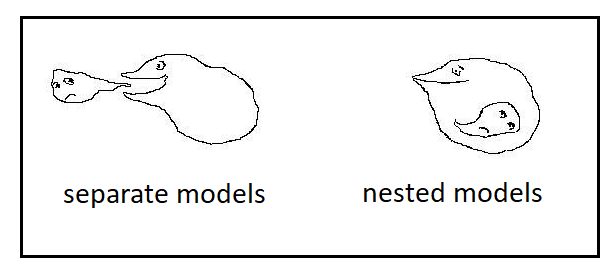
\includegraphics[width=0.5\textwidth]{images/AIC.png}
    \caption{Paveikslėlių numeriai rašomi apačioje, antraštė rašoma apačioje}
    \label{fig:grafikas1}
\end{figure}


Toliau eina tekstas po paveikslėliu.

\subsection{Sąrašai}

Nenumeruojamo sąrašo pavyzdys:
\begin{itemize}
    \item pirmasis elementas;
    \item antrasis elementas.
\end{itemize}

Numeruojamo sąrašo pavydzys:
\begin{enumerate}
    \item lorem ipsum dolor sit amet;
    \item consectetur adipiscing elit;
    \item vivamus a nisl gravida.
\end{enumerate}


\section{Programinio kodo pateikimas}
Šiame skyriuje pateikiamas programinio kodo pateikimo būdas rašto darbe.

\subsection{Algoritmai}

Algoritmai, lygiai taip pat, kaip ir paveikslėliai ar lentelės, yra numeruojami.
Juos būtina paminėti tekste, pvz.:~\ref{alg:gd} naudojamas surasti minimalią funkcijos $\mathcal{L}$ reikšmę.

\begin{algorithm}[h]
\caption{Gradientinio nusileidimo pseudokodas}\label{alg:gd}
\begin{algorithmic}[1]
    \STATE \textcolor{blue}{\texttt{\textbf{\# Darome prielaidą, kad $\mathcal{L}$ apibrėžtas tekste}}}
        \STATE Įeitis: $\mathcal{D}$ -- duomenų rinkinys
        \STATE Įeitis: $\theta_0$ -- parametrų atsitiktinių reikšmių inicializavimas
        \STATE Įeitis: $\gamma$ -- žingsnio dydis, mokymosi greitis (angl.~\textit{learning rate}, \textit{step size})
        \STATE Įeitis: $m$ -- epochų skaičius
        \FOR{$i = 1, 2, \dots, m$}
            \STATE $\theta_i \coloneq \theta_{i-1} - \gamma \nabla_\theta \mathcal{L}(\mathcal{D}, \theta_{i-1})$
            \STATE \textcolor{blue}{\texttt{\textbf{\# Funkcijos $\mathcal{L}$ išvestinė suskaičiuojama automatiškai, autograd pagalba}}}
        \ENDFOR
\end{algorithmic}
\end{algorithm}

\subsubsection{Skyrelio pavyzdys}
\noindent Nebūtina naudoti daug skyrelių (\textit{subsubsections}).

\sectionnonum{Rezultatai ir išvados}
Detaliau, kas turi būti parašyta šiame skyriuje, rasite atitinkamos programos metodiniuose reikalavimuose. 

\printbibliography[title = {Literatūra ir šaltiniai}]


\appendix
\renewcommand{\thesection}{\arabic{section} priedas.}

\section{\phantom{Priedas} Citavimo pavyzdžiai}
Dokumente - \textit{bibliografija.bib}, reikia sudėti visus cituojamus šaltinius ir panaudojus funkciją \textit{\{\textbackslash cite\{cituojamo objekto pavadinimas\}\}} atitinkamas šaltinis bus pridėtas prie literatūros šaltinių sąrašo.


\textit{bibliografija.bib} galima rasti kelių dažniausiai cituojamų šaltinių tipų pavyzdžius:
\begin{itemize}
    \item internetiniai puslapiai (\textit{@online}) \cite{PvzInternetinisPuslapis},
    \item duomenų rinkiniai (\textit{@dataset}) \cite{dataset}
    \item straipsniai (\textit{@article}) \cite{PvzStraipsnLt, PvzStraipsnEn}, 
    \item straipsniai iš konferencijos (\textit{@inproceedings}) \cite{PvzKonfLt, PvzKonfEn}, 
    \item knygos (\textit{@book}) \cite{PvzKnygLt, PvzKnygEn}, 
    \item baigiamieji darbai (\textit{@thesis arba mastersthesis/phdthesis} \cite{PvzMagistrLt, PvzPhdEn})
    \item elektroninės publikacijos (\textit{@misc}) \cite{PvzElPubLt, PvzElPubEn}
\end{itemize}

Taip pat yra pateikti pavyzdžiai - ChatGPT citavimui, tiek bendrai\cite{chatgpt_bendrai}, tiek konkrečiam pokalbiui\cite{chatgpt_pokalbis}.

\end{document}
